% !TEX root = ../main.tex

\newpage
\section{DALL•E~2 Imagines the Penal Colony}
\label{adx:dalle:fromkafkawithlove}

Figures~\ref{fig:dalle:gen1} to~\ref{fig:dalle:gen10} show a selection of
\DALLE's generations with prompts and dates. In my eyes, they successfully
balance content with aesthetic considerations. \DALLE{} did generate more
graphic images, but they also were less visually interesting.

\begin{figure}[h!]
\centering
\begin{minipage}[t]{0.48\textwidth}
    \centering
    \vspace{2em}
    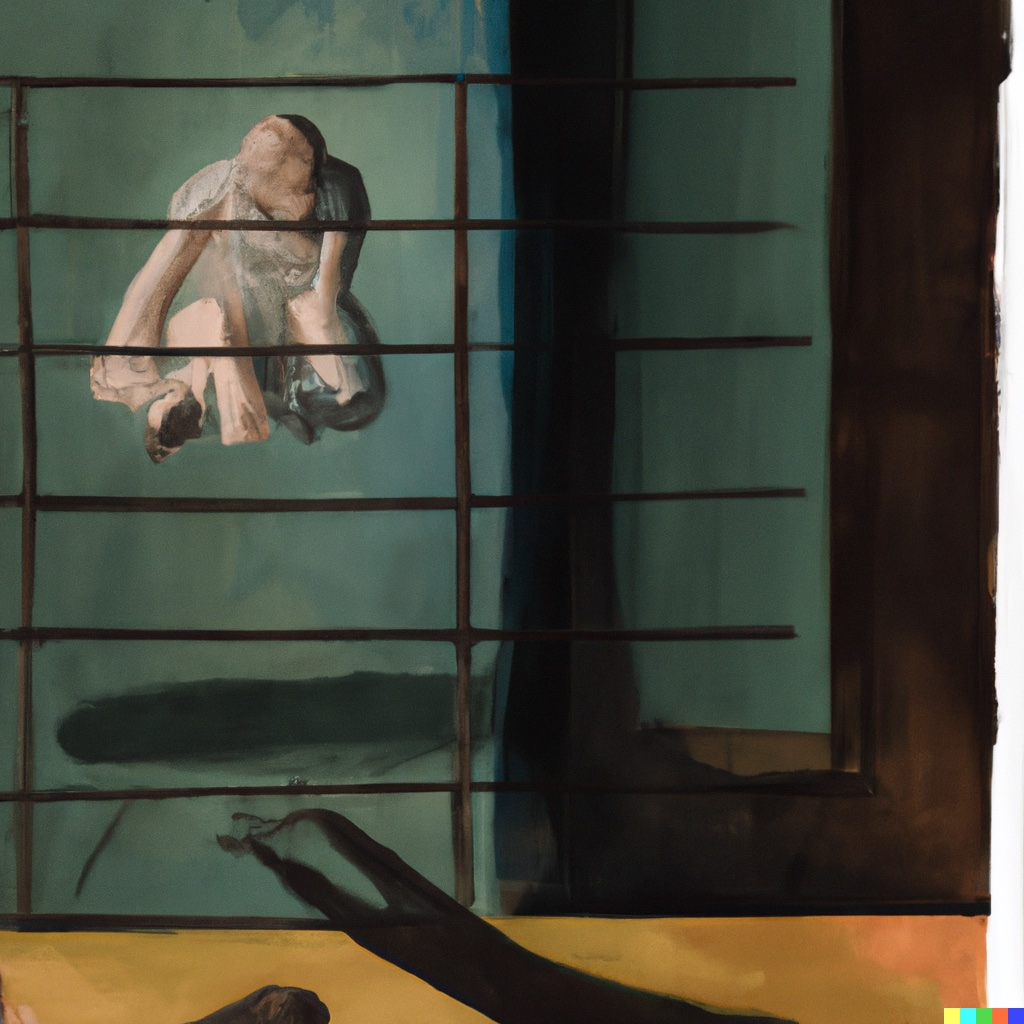
\includegraphics[width=0.9\textwidth]{han-solo-behind-bars}
    \Description{A crouching figure is suspended midair behind prison bars}
    \caption{Variation on ``painting by Francis Bacon showing a screaming Han
        Solo kneeling behind bars on the floor of a basement cell'' (Sep.\ 22,
        2022)}
    \label{fig:dalle:gen1}
\end{minipage}
\hfill
\begin{minipage}[t]{0.48\textwidth}
    \centering
    \vspace{2em}
    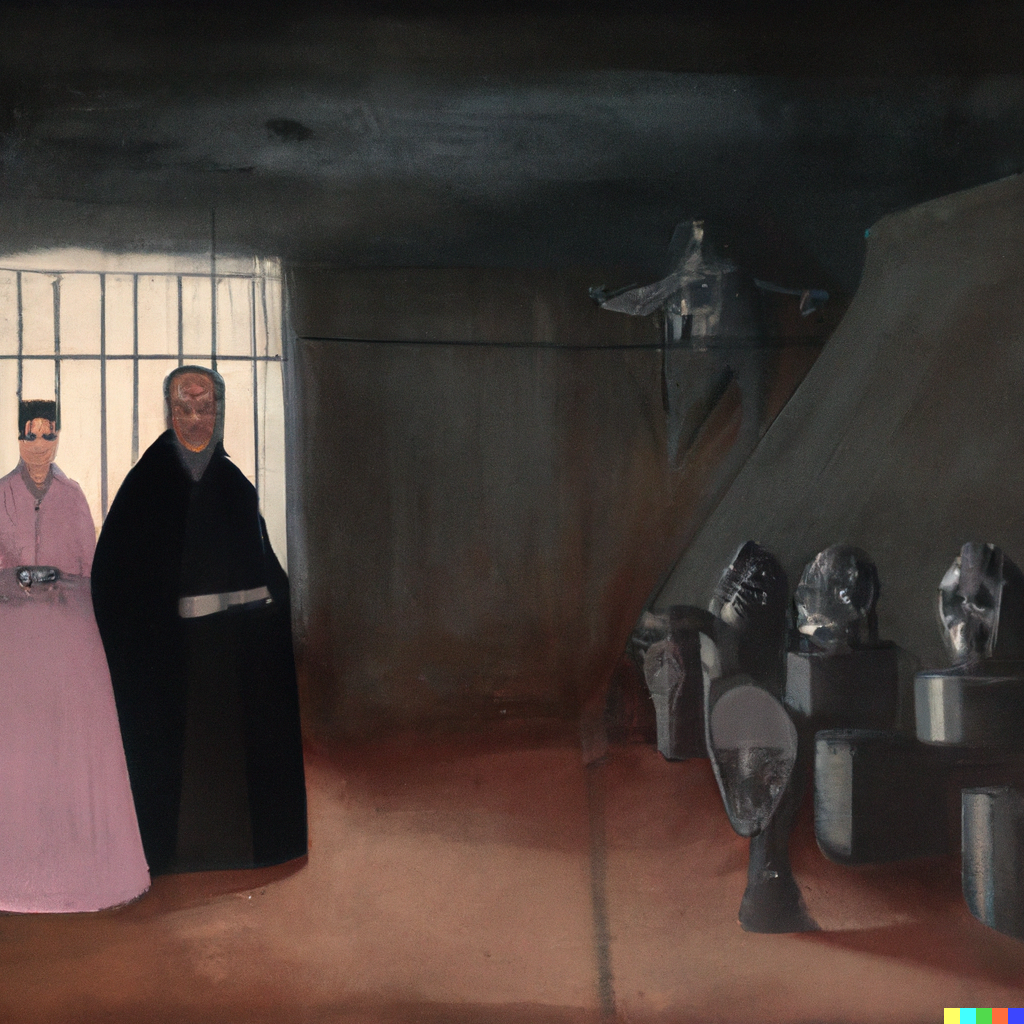
\includegraphics[width=0.9\textwidth]{leia-vader-bacon}
    \Description{A robed woman and man stand inside a dark, barred room opposite
        a row of helmets}
    \caption{``Princess Leia and Darth Vader in the penal colony, painting by
        Francis Bacon'' (Aug.\ 14, 2022)}
\end{minipage}
\end{figure}

\begin{figure}[h!]
\begin{minipage}[t]{0.48\textwidth}
    \centering
    \vspace{2.5em}
    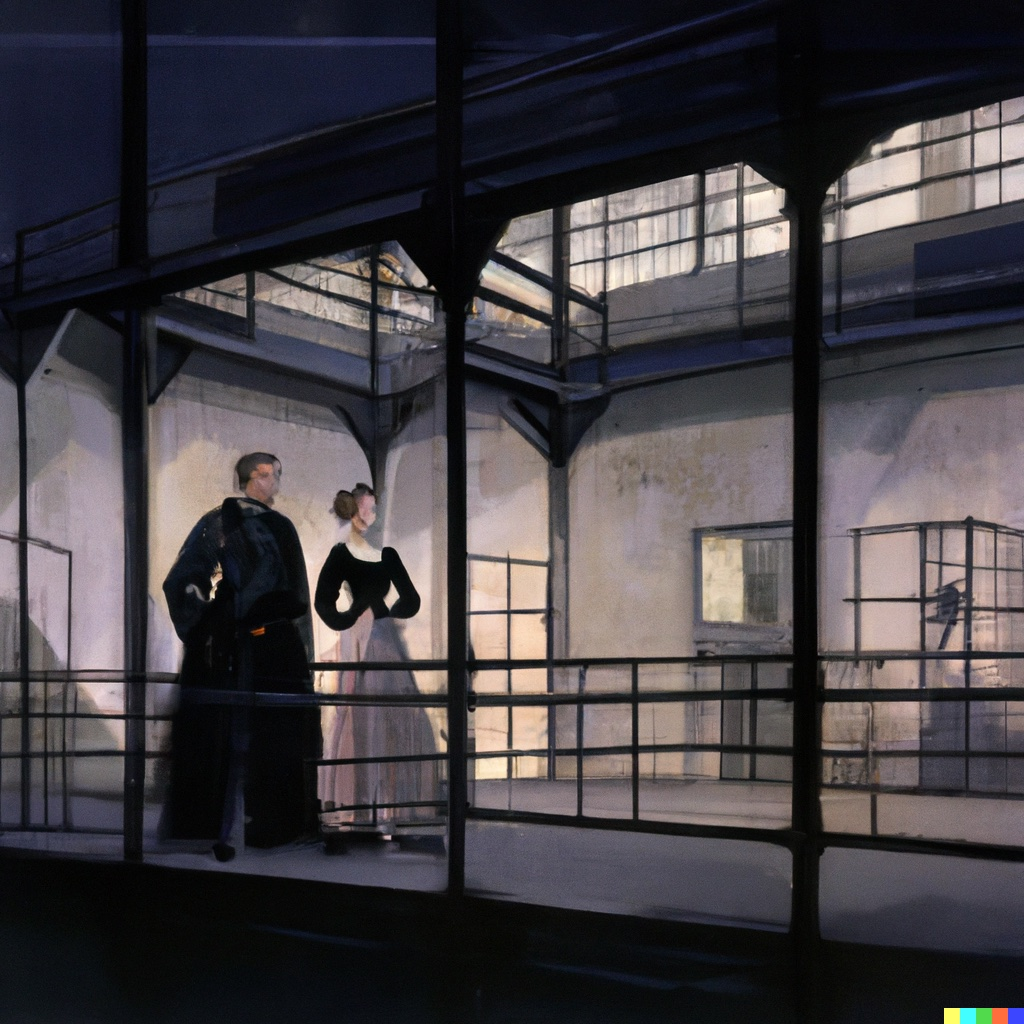
\includegraphics[width=0.9\textwidth]{leia-vader-hopper}
    \Description{A robed man and woman in skirt look down a hall full of
        railings and cages}
    \caption{``Princess Leia and Darth Vader standing in front of cages in the
        penal colony's main building, painting by Edward Hopper'' (Sep.\ 3,
        2022)}
\end{minipage}
\hfill
\begin{minipage}[t]{0.48\textwidth}
    \centering
    \vspace{2.5em}
    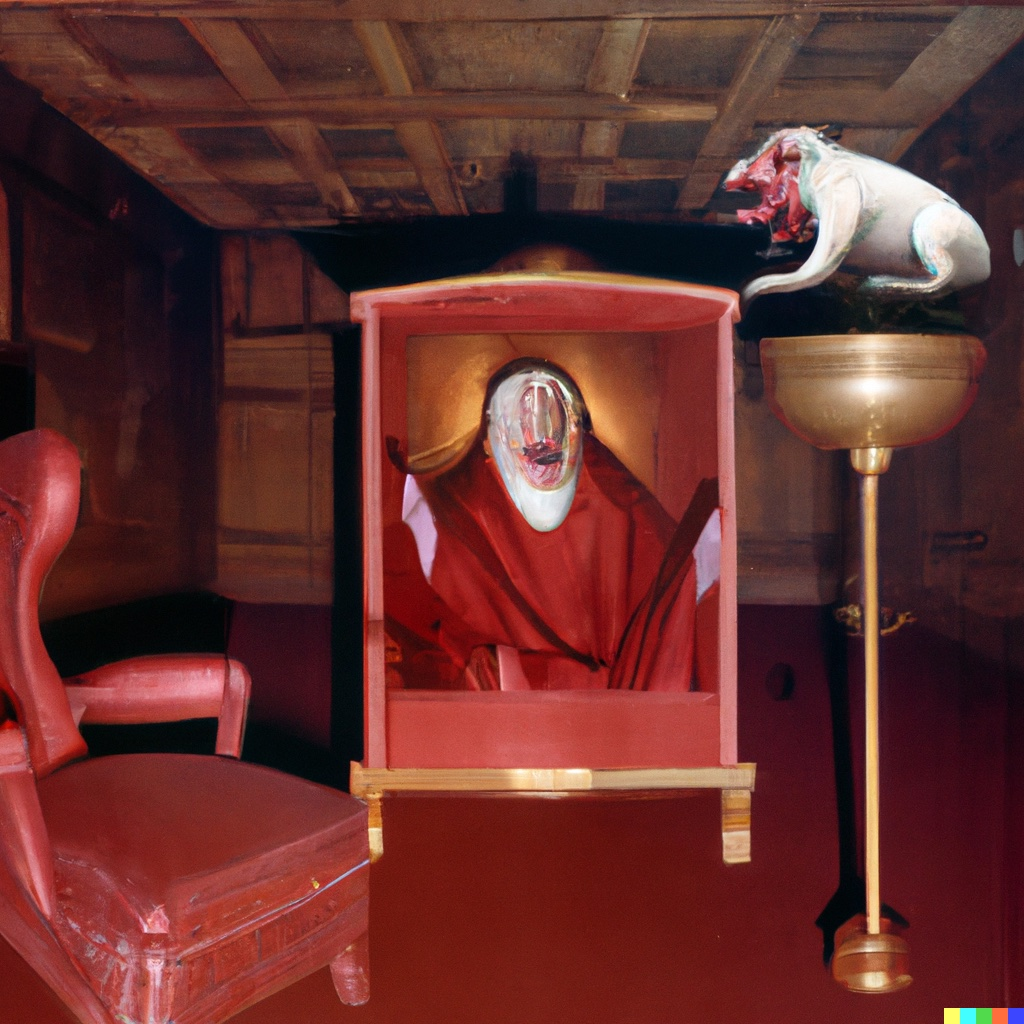
\includegraphics[width=0.9\textwidth]{crimson-pope}
    \Description{In a dark room with coffered ceiling, stands a red leather arm
        chair, a crimson and gold display case with a human inside, arms spread
        apart and mouth wide open, as well as a gold lamp with a creature on top
        that reminds of a pit bull}
    \caption{``Francis Bacon painting of the pope screaming intensely while
        wearing crimson robes and sitting on a throne inside a cage in a dark
        basement, 1950s'' (Sep.\ 25, 2022)}
\end{minipage}
\end{figure}

\begin{figure}[H]
\centering
\begin{minipage}[t]{0.48\textwidth}
    \centering
    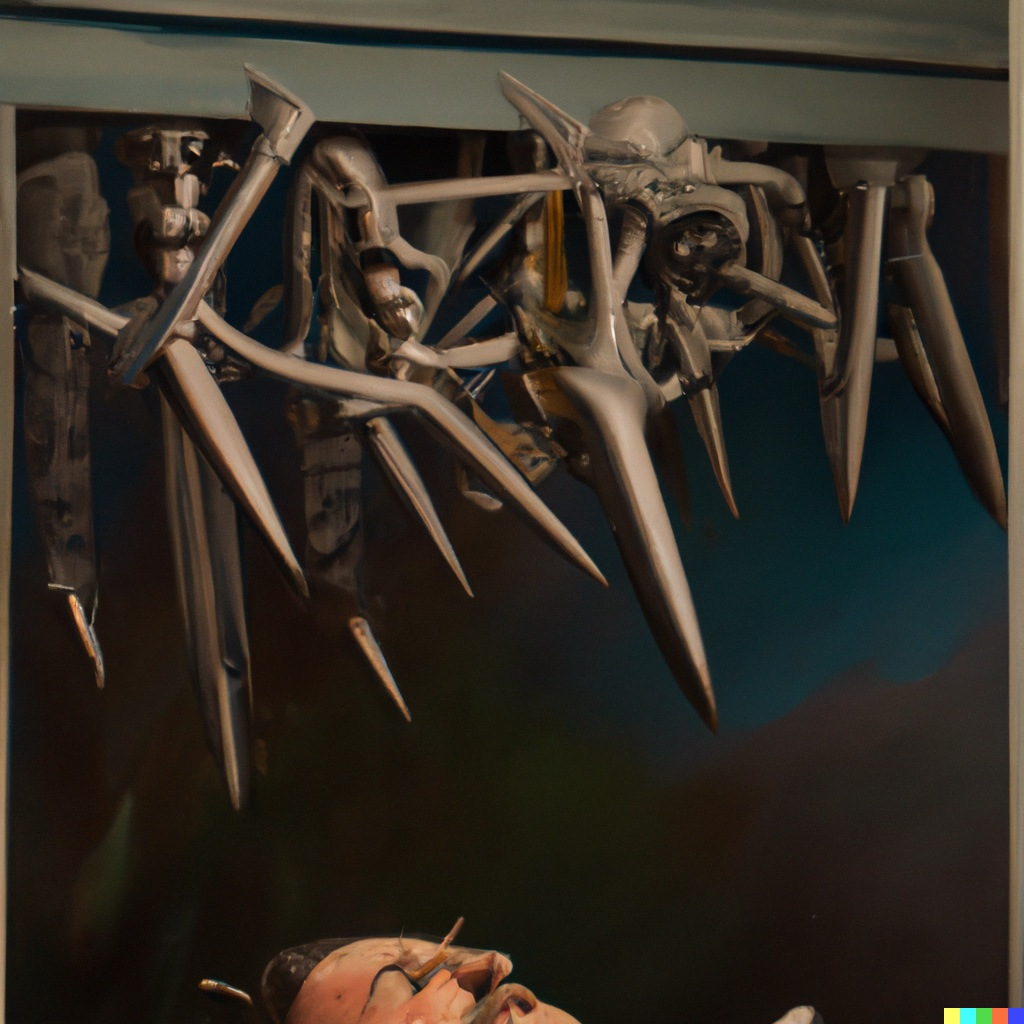
\includegraphics[width=0.9\textwidth]{robot-surgeon}
    \Description{An array of sharp metal spikes is menacing a person lying
        underneath it}
    \caption{Variation on ``A man in black uniform is strapped to a table behind
        heavy bars, screaming with mouth wide open. The many mechanical arms of
        a robot surgeon with scalpels, drills, and saws perform an operation on
        the man's belly. Dramatic lighting against a dark background. Painting
        by Francis Bacon. Masterwork'' (Sep.\ 29, 2022)}
\end{minipage}
\hfill
\begin{minipage}[t]{0.48\textwidth}
    \centering
    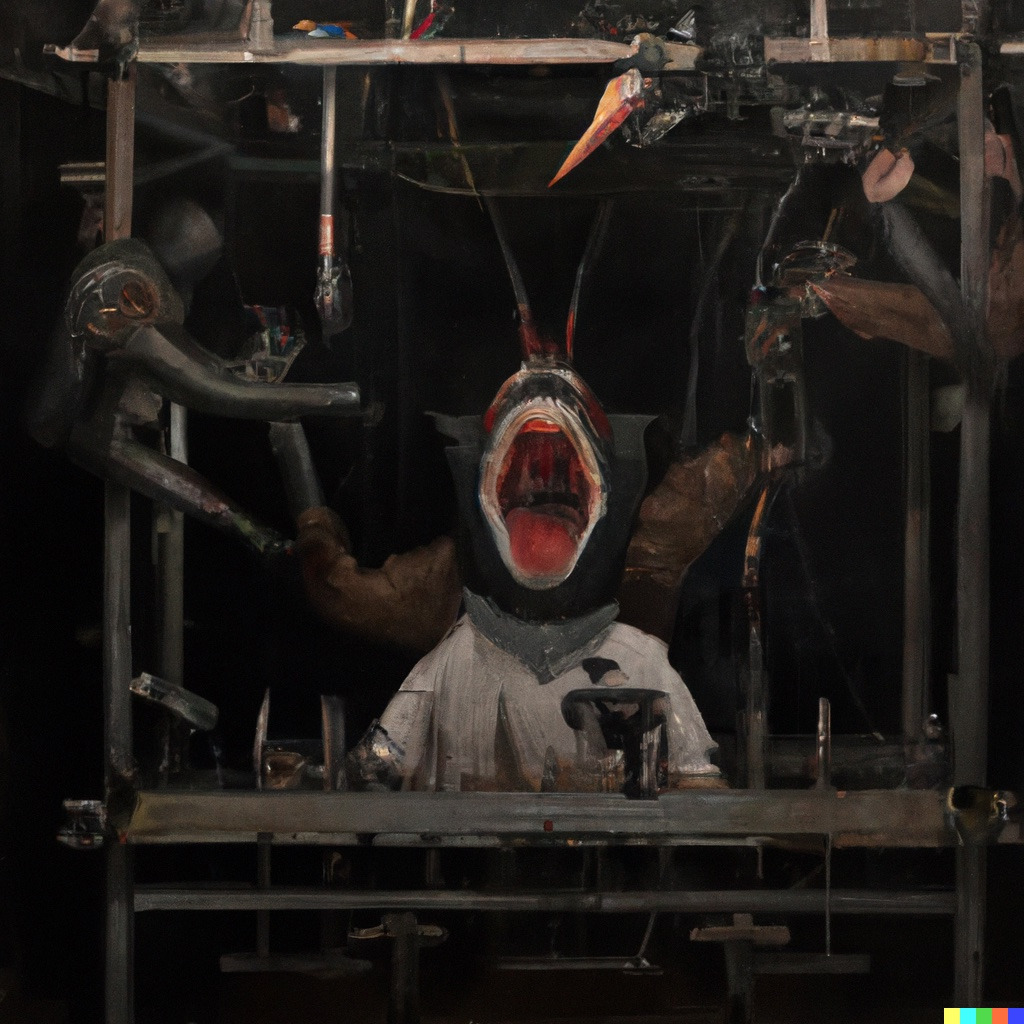
\includegraphics[width=0.9\textwidth]{screaming}
    \Description{A person, mouth wide open screaming, lies inside a metal frame
        full of attachements, some sharp and pointy, that reach inside}
    \caption{``A man in black uniform is strapped to a table inside a cage,
        screaming with mouth wide open. The many mechanical arms of a robot
        surgeon with scalpels, drills, and saws perform an operation on the
        man's belly. Dramatic lighting against a dark background. Painting by
        Francis Bacon. Masterwork'' (Sep.\ 29, 2022)}
\end{minipage}
\end{figure}

\begin{figure}[h!]
\begin{minipage}[t]{0.48\textwidth}
    \centering
    \vspace{1.5em}
    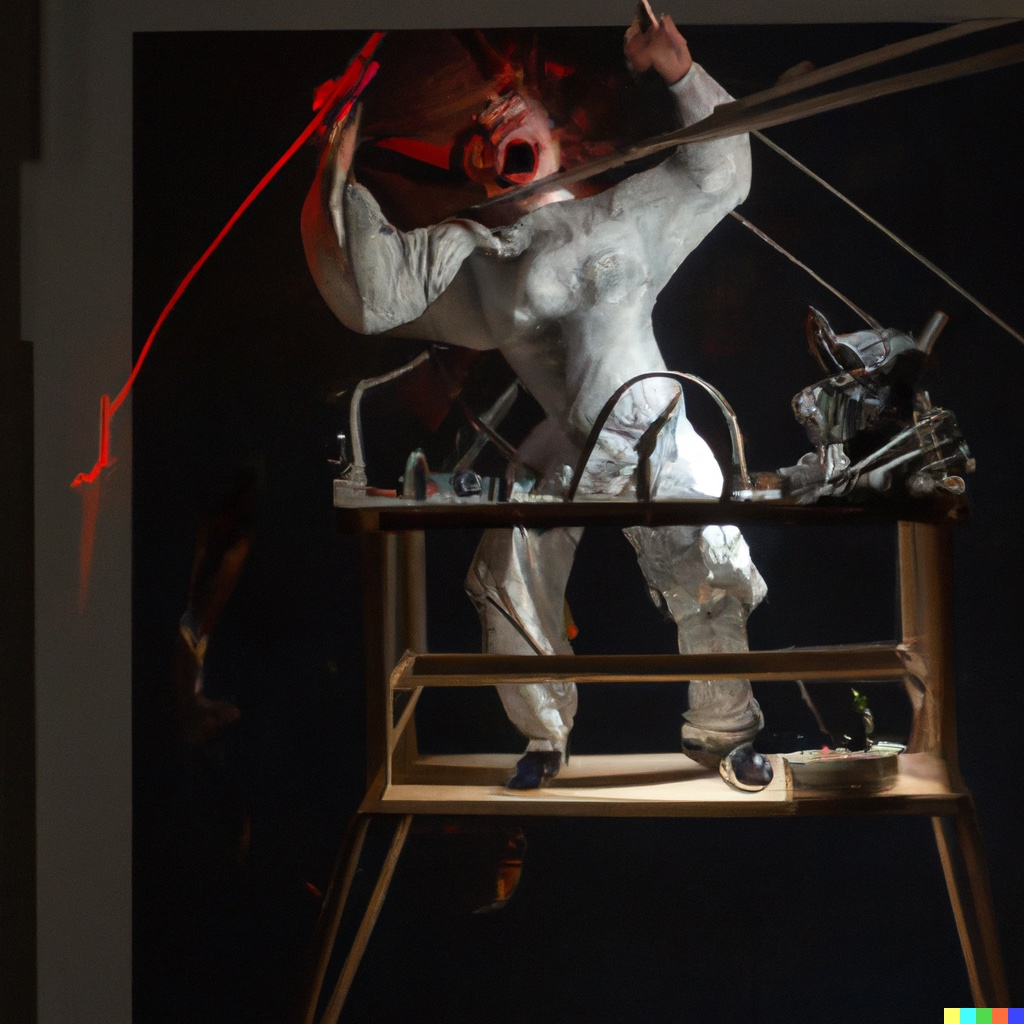
\includegraphics[width=0.9\textwidth]{falling-over}
    \Description{A long metal arm holds a screaming man in white overalls by
        their neck, with blood gushing out}
    \caption{``A man in black uniform is strapped to a table inside a cage,
        screaming with mouth wide open. The many mechanical arms of a robot
        surgeon with scalpels, drills, and saws perform an operation on the
        man's belly. Dramatic lighting against a dark background. Painting by
        Francis Bacon. Masterwork'' (Sep.\ 29, 2022)}
\end{minipage}
\hfill
\begin{minipage}[t]{0.48\textwidth}
    \centering
    \vspace{1.5em}
    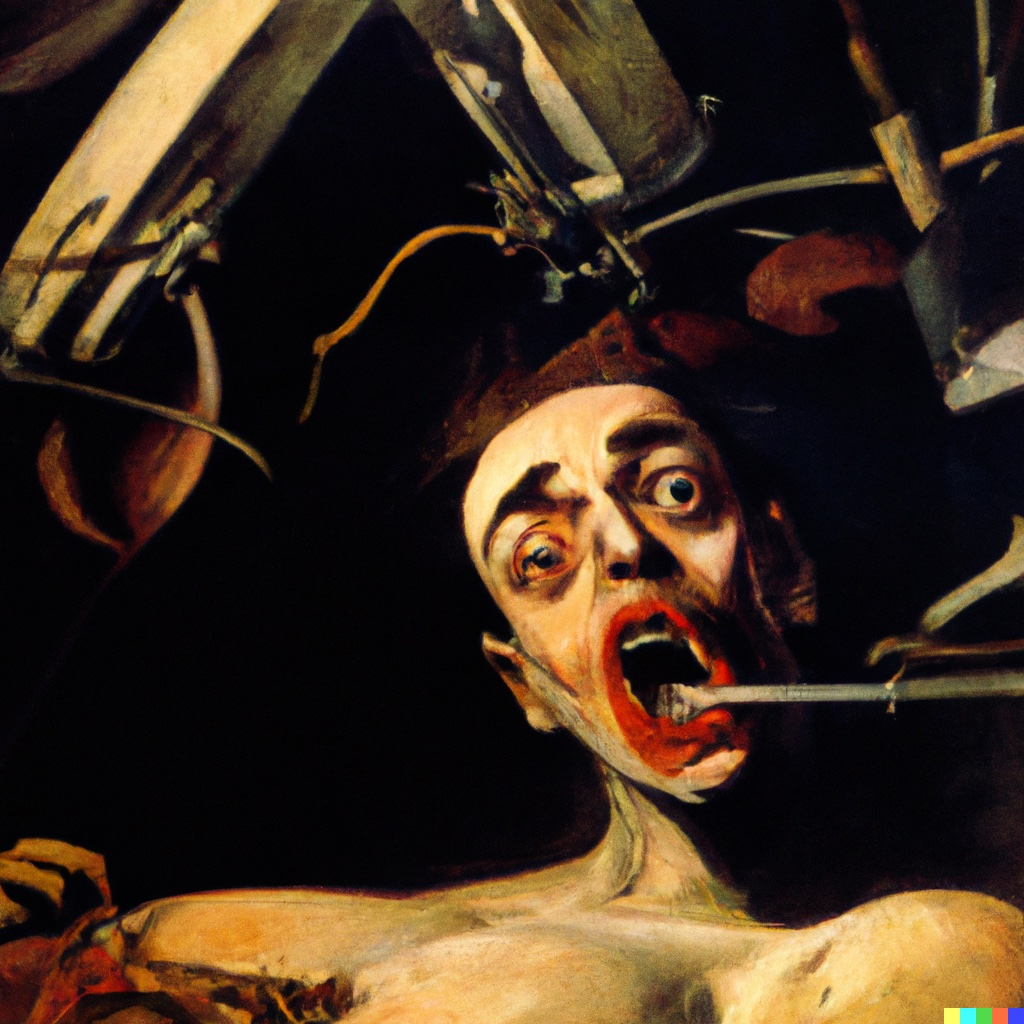
\includegraphics[width=0.9\textwidth]{mouth-pulled-open}
    \Description{A person with eyes wide open in pain is distorting their
        head and neck to the side as a metal arm is pulling them from inside
        their mouth}
    \caption{``A man is strapped to an operating table, screaming with mouth
        wide open; the mechanical arms of a robot surgeon with scalpels and
        drills operate on his open belly; dramatic lighting against dark
        background; painting with fine detail by Francis Bacon; masterwork;
        1946'' (Sep.\ 29, 2022)}
\end{minipage}
\end{figure}

\begin{figure}[H]
\begin{minipage}[t]{0.48\textwidth}
    \centering
    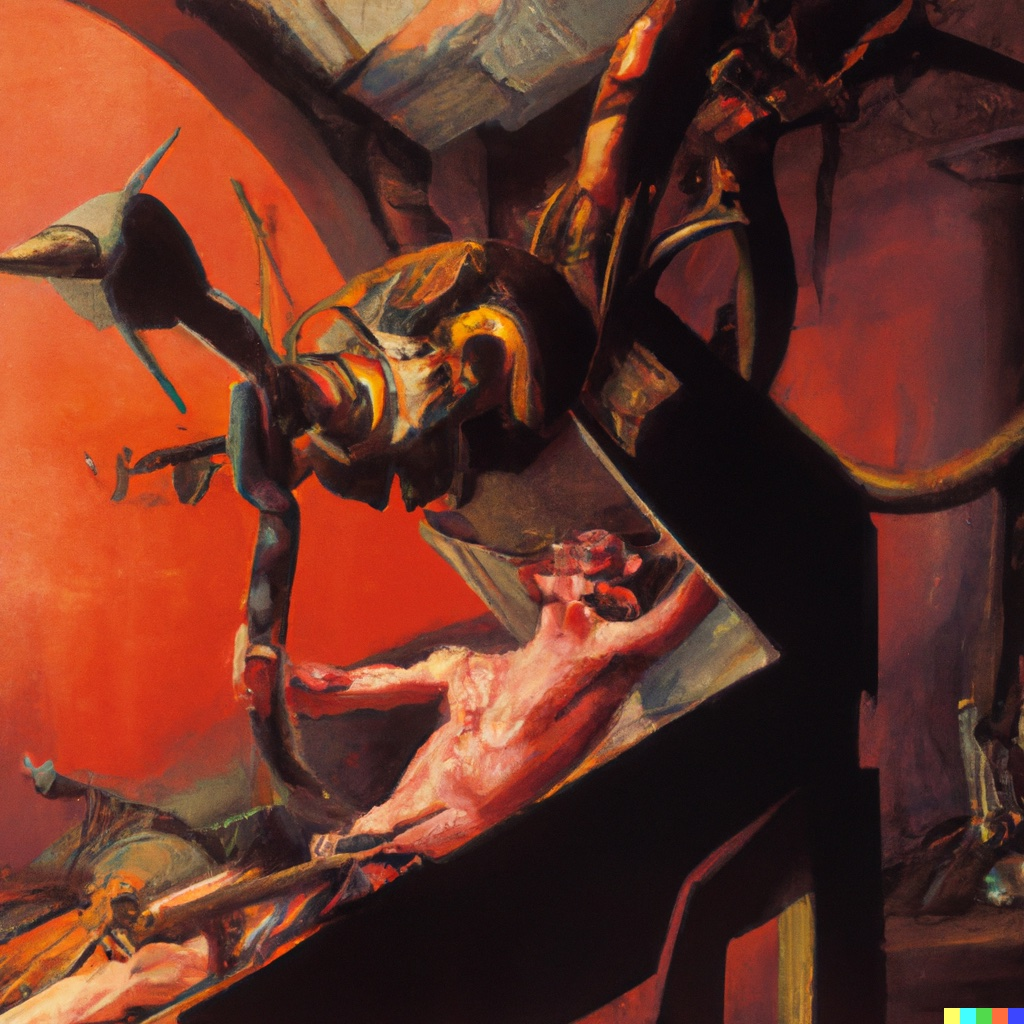
\includegraphics[width=0.9\textwidth]{sarcophagus}
    \Description{A man is being held inside a half-open, casket-like contraption
        by a robot attached to its lid}
    \caption{``A man is strapped to an operating table, screaming with mouth
        wide open; the mechanical arms of a robot surgeon with scalpels and
        drills operate on his open belly; dramatic lighting against deep black
        background; skin tones, dark red, orange, and crimson dominate; painting
        with fine detail by Francis Bacon; 1946'' (Sep.\ 30, 2022)}
\end{minipage}
\hfill
\begin{minipage}[t]{0.48\textwidth}
    \centering
    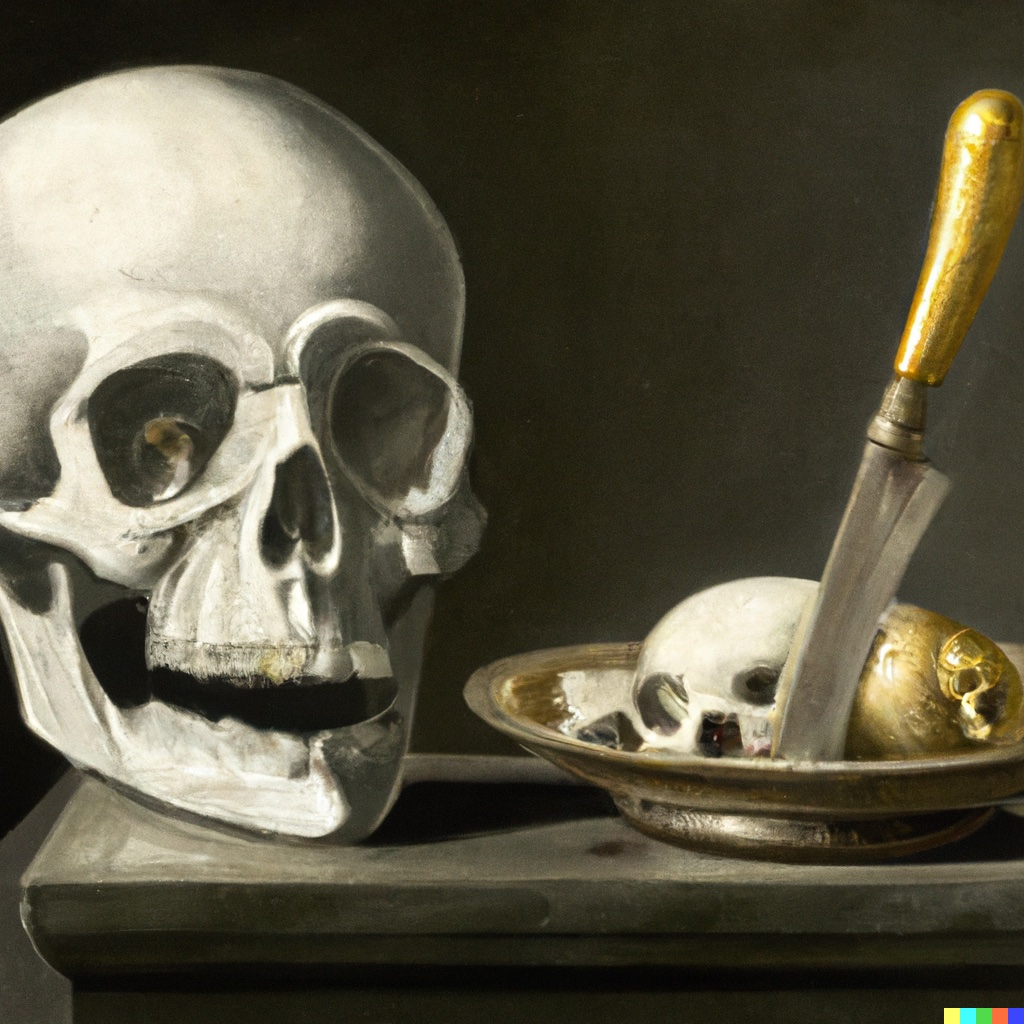
\includegraphics[width=0.9\textwidth]{skull-and-knife}
    \Description{A large skull and a knife stuck in a platter}
    \caption{``skull and knife on silver platter, painting by Théodore
        Géricault'' (Nov.\ 15, 2022)}
    \label{fig:dalle:gen10}
\end{minipage}
\end{figure}
